\chapter{Przygotowanie danych}
Przeprowadzenie procedury testu wiąże się z czynnościami mającymi charakter przygotowawczy. 
Należy do nich min.:
\begin{itemize}
\item stworzenie relacji bazy danych,
\item wypełnienie relacji danymi początkowymi tzw. populacją bazy danych,
\item przygotowanie skryptów testowych.
\end{itemize}
W stworzonym benchmarku operacje te zostały zgrupowane razem w etapie zwanym ,,przygotowanie danych''. 
Niniejszy rozdział omawia ten właśnie etap.
\section{Tworzenie relacji bazy danych}
Jak już zostało wspomniane, model bazy danych jak i model obciążenia, są niezależne
od konkretnego DBMS. Pierwszym momentem, w którym następuje związanie tych modeli
z konkretnym DBMS, jest właśnie moment tworzenia relacji w bazie danych.
Pomimo istnienia języka SQL poszczególne DBMS różnią się pomiędzy sobą dostępnymi typami danych.
Typy te są szczególnie widoczne w zapytaniach tworzących relacje. W omawianym benchmarku
do tworzenia skryptów tworzących relacje została użyta biblioteka Hibernate~\cite{Hibernate1} 
oraz Hibernate Annotations~\cite{HibernateAnn1}.
Proces tworzenia relacji składa się z następujących etapów:
\begin{enumerate}
\item Wygenerowanie na podstawie modelu bazy danych klas -- zgodnych ze
specyfikacją Hibernate Annotations.
\item Kompilacja klas.
\item Załadowanie klas do biblioteki Hibernate. 
\item Wygenerowanie skryptów przy pomocy biblioteki Hibernate.
\item Utworzenie relacji w bazie danych.
\end{enumerate}
\section{Generowanie populacji bazy danych}\label{sect:populationgeneration}
Aby móc przeprowadzić testy na bazie danych niezbędne jest by w bazie tej znajdowały się dane.
Dane te powinny charakteryzować się szeregiem własności:
\begin{itemize}
\item odpowiednią proporcją pomiędzy liczbą krotek w poszczególnych relacjach,
\item odpowiednią zawartością wartości pustych w poszczególnych kolumnach,
\item monotonicznością lub jej brakiem dla poszczególnych atrybutów,
\item zakresem dopuszczalnych wartości np.: w przypadku typów wyliczeniowych, czy kluczy obcych.
\end{itemize}
Na podstawie informacji z modelu bazy danych, oraz wartości parametrów skalujących z modelu 
testu, relacje bazy danych wypełniane są krotkami. Proces ten w ogólności nie jest trywialny -- 
powstaje tutaj szereg problemów, jak chociażby generowanie złożonych kluczy głównych, 
czy złożonych kluczy obcych. Już samo istnienie referencji na inne relacje wymusza uszeregowanie relacji np.: 
aby wprowadzić wartość dla klucza obcego w relacji A, muszą istnieć dane w relacji B.

Algorytm tworzenia populacji
\begin{enumerate}
\item Uszereguj relacje -- postępuj zgodnie z algorytmem poszukiwania cykli w grafie.
(Kolejność usuwania relacji w algorytmie jest kolejnością posortowania relacji.)
Mechanizm tworzenia populacji benchmarku, nie radzi sobie z cyklami -- poza cyklami na ,,siebie''.
Cykl na ,,siebie'' jest to klucz obcy na własne kolumny. Przykładem cyklu z jakim mechanizm sobie nie radzi,
może być cykl pomiędzy trzema relacjami A, B i C, gdzie relacja A posiada klucz obcy na B, B na C oraz C na A. 
Warto jednak zauważyć, że istnienie zależności cyklicznych zarówno w programowaniu obiektowym, 
jak i w bazach danych, jest przykładem złej praktyki. Praktycznie każdą zależność cykliczną 
idzie przekształcić na zależność jednokierunkową.

\item Utwórz generatory krotek relacji.
\item Wyszukaj wszystkie kolumny każdej relacji używane jako klucze obce -- w ten sposób określa się, 
które kolumny mają mieć wartości generowane na podstawie wartości innych kolumn. Jeżeli bowiem kolumna
jest kluczem obcym na inną kolumnę, to jej wartości muszą pochodzić z tej właśnie kolumny.
\item Utwórz struktury buforujące dla poszczególnych relacji/generatorów relacji.
\item Ustaw klucze obce w generatorach relacji.
\item Generuj dane.
\end{enumerate}
\section{Przygotowanie skryptów testowych}
\subsection{Wstęp}
Ważnym etapem przygotowywania danych jest utworzenie skryptów testowych, które następnie
w procedurze testu będą wykonywane na poszczególnych RTE. Liczba potrzebnych skryptów
jest równa liczbie RTE niezbędnych w procedurze testu. Dla każdego skryptu,
na podstawie analizy modelu obciążenia, a także parametrów skalujących z modelu testu, 
określana jest liczba operacji i transakcji do przetestowania na pojedynczym RTE.
Następnie dla każdego RTE tworzony jest niezależnie skrypt testowy –- o tej samej strukturze, 
lecz różnych danych, dla poszczególnych operacji.
\subsection{Budowa skryptu testowego}\label{sub:testscript}
Na rys.~\ref{rys:test-script} przedstawiono przykładowy skrypt testowy przeznaczony do wykonania na jednym z RTE. 
Rzeczywisty skrypt jest oczywiście bardziej złożony, posiada min.: wielokrotnie więcej operacji SQL. 
Rzeczywisty skrypt generowany jest dla każdego RTE przez serwer, przed rozpoczęciem testu.
Zawiera on zestaw testów dla poszczególnych operacji i transakcji opisanych w modelu obciążenia. Każda 
komenda ,,nie SQL'' poprzedzona jest znakiem ,,$>$''. Poniżej wyjaśniono wszystkie te komendy:
\begin{itemize}
\item $>$s -- wysłanie z RTE sygnału synchronizującego do serwera, serwer oczekuje na sygnały synchronizujące od
wszystkich RTE biorących udział w teście, po czym odsyła do nich własny sygnał synchronizujący,
\item $>$w -- oczekiwanie przez klienta RTE na sygnał synchronizujący z serwera, dalsze wykonywanie skryptu testowego jest
zawieszane,
\item $>$t -- pomiar czasu na RTE i zapisanie go do pliku ,,test.time'',
\item $>$c -- wykonanie operacji commit,
\item $>$l -- wykonanie operacji SQL wymagającej wstawienia obiektu typu LOB(\english{large object}) 
czyli BLOB (\english{binary large object}) lub CLOB (\english{character large object}). 
Obiekty tego typu nie są umieszczane bezpośrednio w skrypcie, lecz w 
dwóch odrębnych plikach ,,test.blob'' oraz ,,test.clob''. Interpreter skryptu, 
gdy napotka komendę rozpoczynającą się od litery~,,l'' analizuje ją do pierwszego znaku~,,:''. 
Znakiem ,,,'' rozdzielone są sekcje dotyczące kolejnych obiektów lob. 
Pierwsza litera każdej sekcji ,,mówi'' czy sekcja dotyczy obiektu typu BLOB czy CLOB. 
Każda sekcja zawiera także informacje o długości obiektu. Kolejność sekcji odpowiada kolejności
występowania odwołań do obiektów lob w komendzie języka SQL, umieszczonej po pierwszym znaku~,,:''. 
Miejsca, w których obiekty te mają się znaleźć oznaczone są znakiem~,,?''. 
W zależności od typu sterownika wstawianie obiektów LOB odbywa się albo poprzez funkcje 
,,setBinaryStream'', ,,setCharacterStream'' lub ,,setBlob'', ,,setClob''.
\end{itemize} 

\begin{figure}[t]
{\footnotesize
$>$s /*Wysłanie sygnału do serwera*/\\
$>$w /*Oczekiwanie na sygnał z serwera*/\\
$>$t /*Pomiar czasu*/\\
select * from tbl\_customer where customer\_id = 12\\
$>$t \\
$>$s \\
$>$w \\
$>$t \\
insert into tbl\_subscriber(email) values('janek@wp.pl')\\
$>$t \\
$>$r /*Operacja rollback*/\\
$>$t \\
update tbl\_person set sex = 'male‘ where person\_id = 7\\
delete from tbl\_subscriber where email = 'mirek@wp.pl'\\
$>$t\\
$>$s\\
$>$w\\
$>$t\\
l,b1200,c123:insert into tbl\_products values('name',?,?)\\
$>$t\\
$>$c /*Operacja commit*/\\
$>$s\\ 
}
\caption{Przykładowy skrypt testowy}\label{rys:test-script}
\end{figure}
Na uwagę zasługuje fakt, iż para operacji ,,$>$s $>$w'' występuje poza wysłaniem ostatniego sygnału 
synchronizującego do serwera, zawsze razem. Pierwsza operacja powoduje wysłanie z RTE sygnału 
synchronizującego do serwera, druga zaś wstrzymuje wykonanie testu do momentu wysłania sygnału 
synchronizującego w odwrotnym kierunku. Serwer odsyła każdorazowo taki sygnał, gdy otrzyma 
sygnały synchronizujące od wszystkich RTE biorących udział w teście. Taki zabieg umożliwia synchronizację 
wykonywanych na poszczególnych RTE skryptów testowych. Synchronizacja taka jest wykonywana 
przed każdym testem. Po zakończeniu testu, każdy RTE wysyła do serwera ostatni sygnał synchronizujący, 
gdy serwer otrzyma taki sygnał od każdego RTE –- ,,wie'', że procedura testowa zakończyła się.
Ponadto, jeżeli w trakcie wykonywania którejś z komend języka SQL wystąpi wyjątek, to zostanie 
on przechwycony i zapisany w pliku ,,test.error'', wraz z numerem linii skryptu, którego błąd dotyczył. 
Zamieszczone w przykładzie komentarze typu /*…*/ w rzeczywistym skrypcie nie występują. 
\subsection{Typy testów}\label{sect:testtypes}
Skrypt testowy składa się z czterech typów testów:
\begin{itemize}
\item obciążeniowego operacji,
\item obciążeniowego transakcji,
\item proporcjonalnościowego operacji,
\item proporcjonalnościowego transakcji.
\end{itemize}

Testy obciążeniowe operacji to testy, w których występują operacje zdefiniowane w modelu obciążeniowym.
Podczas tego typu testów na wszystkich RTE równocześnie wykonywane są operacje \textit{tylko} jednego typu.
Testy takie pozwalają przyjrzeć się dokładnie jednemu typowi operacji, nie uwzględniają jednak całej złożoności
modelu obciążeniowego.

Testy obciążeniowe transakcji to testy, w których na wszystkich RTE równocześnie wykonywane są transakcje \textit{tylko} jednego typu.
Testy takie pozwalają przyjrzeć się dokładnie jednemu typowi transakcji, nie uwzględniają jednak całej złożoności
modelu obciążeniowego.

Testy proporcjonalnościowe operacji to testy, w których na wszystkich RTE równocześnie wykonywana jest pewna 
,,proporcjonalnościowa mieszanka'' operacji. Na każdym RTE kolejność operacji jest losowa, proporcjonalność zaś
wynika z obliczeń dokonywanych na podstawie modelu obciążeniowego.

Testy proporcjonalnościowe transakcji to testy, w których na wszystkich RTE równocześnie wykonywana jest pewna 
,,proporcjonalnościowa mieszanka'' transakcji. Na każdym RTE kolejność transakcji jest losowa, proporcjonalność zaś
wynika z obliczeń dokonywanych na podstawie modelu obciążeniowego.

\subsection{Podsumowanie}
Reasumując, w procedurze generowana skryptów testowych, dla każdego RTE biorącego 
udział w teście zostają wygenerowane trzy pliki: ,,test.script'', ,,test.blob'' oraz ,,test.clob''.
Pliki te wraz ze sterownikiem jdbc (,,jdbc.jar''), a także z opisem parametrów połączenia i dialektem (plik ,,test.properties''), 
pakowane są do archiwum ,,test.zip'' (zob. rys.~\ref{rys:testzip}). Ostatecznie otrzymujemy kolekcje plików zip 
–- po 1 na każdego klienta RTE, który ma wziąć udział w teście.
\begin{figure}[h]
\begin{center}
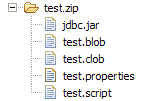
\includegraphics[width=0.4\linewidth]{figures/testzip.png}
\end{center}
\caption{Struktura pliku ,,test.zip''}\label{rys:testzip}
\end{figure}
Ostatnim etapem generacji skryptów testowych jest wygenerowanie pliku ,,test.metadata''. 
Plik ten zawiera informacje dla serwera niezbędne w procesie zbierania i analizy wyników testu.
Plik ten nie jest wysyłany do RTE, serwer przechowuje go lokalnie u siebie. 



